\documentclass[twocolumn]{article}
\usepackage[spanish]{babel}
\usepackage[utf8]{inputenc}
\usepackage{amssymb}
\usepackage{graphicx}
\usepackage{verbatim}
\usepackage{algorithmic}
\usepackage{enumitem}
\setlist{nolistsep}




\author{
Nombre:....................................... \\
    Departamento de Informática y Sistemas \\
    Universidad EAFIT \\
}
\title{
    Estructuras de Datos 2 - ST0247 - 032 \\
    Examen Parcial 2 (jueves)
}
\date{
    Mayo 11, 2017
}

\begin{document}
\vspace{-5cm}
\maketitle


\section*{Criterios de calificación}

\begin{itemize}
\item Selección múltiple con única respuesta
\begin{itemize}
\item Respuesta correcta: 100\%
\item Respuesta incorrecta: 0\%
\end{itemize}

\item Completar código
\begin{itemize}
\item Respuesta correcta 100\%
\item Respuesta incorrecta o vacía 0\%
\end{itemize}
\end{itemize}

\textbf{NOTAS IMPORTANTES:}
\begin{itemize}
	\item Responda en la hoja de PREGUNTAS
	\item Marque la hoja de PREGUNTAS
\end{itemize}

\section{Dividir y Conquistar 20\%}
Hoy es el último día de Dayla y Kefo en el Colegio y hoy presentan su último examen de Matemáticas. Casi todos los puntos son simples excepto por uno. Supongamos que nos entregan una función $f(x)$ \textit{unimodal} en un intervalo $I: [l, r]$. Una función unimodal es aquella que siempre es creciente hasta un punto y luego decreciente (o viceversa). La idea es encontrar el máximo  de esa función en el intervalo $I$. 

Dayla y Kefo aprovecharon y utilizaron su código de \textit{ternary search} para determinar el máximo. \textit{Ternary search} determina si el máximo no se puede encontrar en el primer tercio del intervalo o si no se puede encontrar en el último tercio
del intervalo, luego repite el proceso en los dos tercios que no fueron descartados. Desafortunadamente, ambos se dieron cuenta que su código no andaba bien y te lo entregan a ti para que lo corrijas. En el examen, la función que les entregaron fue $f(x) = 2x^2 - 12x + 7$.\\

\textbf{Pista: } Como la función $f(x)$ es \textit{unimodal}, si tomamos dos puntos $m_1$ y $m_2$ en el intervalo: $l < m_1 < m_2 < r$, entonces hay 3 posibilidades

\begin{enumerate}
\item Si $f(m_1) < f(m_2)$, entonces el máximo no está en el tercio de la izquierda, sino en los otros dos tercios.
\item Si $f(m_1) > f(m_2)$, entonces el máximo no está en el tercio de la derecha, sino en los otros dos tercios.
\item Si $f(m_1) = f(m_2)$, entonces el máximo es $m_1$.\\
\end{enumerate}

\textbf{Pista 2: } Elija así los puntos \texttt{m1} y \texttt{m2}: \\

\begin{itemize}
\item $m1 = l + (r-l)/3$
\item $m2 = r - (r-l)/3$
\end{itemize}

{\small
\begin{verbatim}
double f(double x){
    return 2 * x * x - 12 * x + 7;}

double buscarMax(double left, double right) {
    if (right == left) 
        return left; 
    leftThird = (2*left + right)/2;
    rightThird = (left + 2*right)/3;
    if (f(leftThird) < f(rightThird))
        return ternarySearch(leftThird, right); 
    else
        return ternarySearch(left, rightThird);
} 
\end{verbatim}
}

\noindent
1.1 (10\%) ¿Cómo se soluciona el error en el código de Dayla y Kefo?

\begin{enumerate}[label=\Alph*]
\item El error se soluciona cambiando \texttt{ leftThird = (2*left + right)/2} por 
\texttt{ leftThird = (2*left + right)/3}\\
\item El error se soluciona cambiando \texttt{ rightThird =(left + 2*right)/3} por
\texttt{ leftThird = (left + 2*right)/2}\\
\item El error se soluciona cambiando \texttt{ leftThird = (2*left + right)/2} por
\texttt{ leftThird = (2+left + right)/2}\\
\item El error se soluciona cambiando \texttt{ leftThird = (left + 2*right)/3} por
\texttt{ leftThird = (left + 2+right)/3}\\
\end{enumerate} 

%A.  El error se soluciona cambiando \texttt{ leftThird = (2*left + right)/2} por 
%\texttt{ leftThird = (2*left + right)/3}

\noindent
1.2 (10\%) Además de corregir el error anterior, ¿qué más se debe modificar para calcular el mínimo de la función en lugar del máximo?

\begin{enumerate}[label=\Alph*]
\item Se cambia \texttt{if(f(leftThird) $<$ f(rightThird))} por \texttt{if(f(leftThird) $>$ f(rightThird))}\\
\item Se cambia \texttt{if(f(leftThird) $<$ f(rightThird))} por \texttt{if(f(leftThird) !$=$ f(rightThird))}\\
\item Se cambia \texttt{if(f(leftThird) $>$ f(rightThird))} por \texttt{if(f(leftThird) $<$ f(rightThird))}\\
\item Se cambia \texttt{(left + right)/2} por \texttt{(left + right)/3}
\end{enumerate}

%A, se cambia < por >.

\section{Prog. Dinámica 30\%}
La distancia de Levenshtein es el número mínimo de operaciones requeridas para transformar una cadena de caracteres en otra. Se entiende por operación, una inserción, eliminación o la sustitución de un carácter. Es útil en programas que determinan cuán similares son dos cadenas de caracteres, como es el caso de los correctores de ortografía. Como un ejemplo, la distancia de Levenshtein entre ``casa'' y ``calle'' es de $3$ porque se necesitan al menos tres ediciones elementales para cambiar uno en el otro:

\begin{enumerate}
   \item casa $\rightarrow$ cala (sustitución de 's' por 'l')
  \item  cala $\rightarrow$ calla (inserción de 'l' entre 'l' y 'a')
   \item calla $\rightarrow$ calle (sustitución de 'a' por 'e')
\end{enumerate}


A continuación está una implementación del algoritmo en Java:

{\small
\begin{verbatim}
int minimum(int a, int b, int c) {                            
  return Math.min(Math.min(a, b), c);                                      
}                                                                            
                                                                                
int Levenshtein(String lhs, String rhs) {      
  int[][] distance = new int[lhs.length() + 1]
                            [rhs.length() +1];                                   
  for (int i = 0; i <= lhs.length(); i++)                                 
    distance[i][0] = i;                                                  
  for (int j = 1; j <= rhs.length(); j++)                                 
    distance[0][j] = j;                                                                     
  for (int i = 1; i <= lhs.length(); i++)                                 
    for (int j = 1; j <= rhs.length(); j++)                             
     distance[i][j] = minimum(                                        
      distance[i - 1][j] + 1,                                  
      distance[i][j - 1] + 1,                                  
      distance[i - 1][j - 1] + 
      ((lhs.charAt(i - 1) == rhs.charAt(j - 1)) ? 0 : 1));                                                           
  return distance[lhs.length()][rhs.length()];                          
}                                                                            
\end{verbatim}
}


En Java, el operador incógnita (?) funciona de la siguiente forma: Si \texttt{algo} es verdadero, entonces retorna un \texttt{valor},
de lo contrario retorna otro \texttt{valor}, así:
\texttt{algo? un valor : otro valor}.


(15 \%) Complete la siguiente tabla, siguiendo el algoritmo de programación dinámica de la distancia de Levenshtein:\\

\begin{tabular}{| l  | l  | l  | l  | l  | l  | l |}
\hline
  & & c & a & l & l & e \\
 \hline
  & &  &  &  &  &  \\
  \hline
c & &  &  &  &  &  \\
\hline
a & &  &  &  &  &  \\
\hline
s & &  &  &  &  &  \\
\hline
a & &  &  &  &  &  \\
\hline
\end{tabular}

%  	  	c 	a 	l 	l 	e
%   	0 	1 	2 	3 	4 	5
% c 	1 	0 	1 	2 	3 	4
% a 	2 	1 	0 	1 	2 	3
% s 	3 	2 	1 	1 	2 	3
% a 	4 	3 	2 	2 	2 	3

(15 \%) Complete la siguiente tabla, siguiendo el algoritmo de programación dinámica de la distancia de Levenshtein, para encontrar
la distancia entre madre y mama:\\

\begin{tabular}{| l  | l  | l  | l  | l  | l  | l |}
\hline
  & & m & a & d & r & e \\
 \hline
  & &  &  &  &  &  \\
  \hline
m & &  &  &  &  &  \\
\hline
a & &  &  &  &  &  \\
\hline
m & &  &  &  &  &  \\
\hline
a & &  &  &  &  &  \\
\hline
\end{tabular}


\section{Algo. voraces 30\%}
El algoritmo de Dijkstra sirve para encontrar el camino más corto
de un vértice a todos los demás de un grafo. A continuación una
implementación en Java.

{\small
\begin{verbatim}
int minVertex (int [] dist, boolean [] v) {
 int x = Integer.MAX_VALUE; //Infinity
 int y = -1;   
 for (int i=0; i<dist.length; i++) 
  if (!v[i] && dist[i]<x) 
     y=i; x=dist[i];
 return y;
}
      
int [] dijsktra(Graph dg, int source) {
  int [] dist = new int [dg.size()]; 
  int [] pred = new int [dg.size()]; 
  boolean [] visited = new boolean [dg.size()]; 
  for (int i=0; i<dist.length; i++) 
    dist[i] = Integer.MAX_VALUE; 
  dist[source] = 0;
  for (int i=0; i<dist.length; i++) {
    int next = minVertex (dist, visited);
    visited[next] = true;
    ArrayList<Integer> n =
        dg.getSuccessors (next); 
    for (int j=0; j<n.size(); j++) {
      int v = n.get(j);
      int d = dist[next] + 
          dg.getWeight(next,v);
      if (dist[v] > d) {
        dist[v] = d;
        pred[v] = next;
      }}}
  return pred;  
}
\end{verbatim}
}

Considere el siguiente grafo:

\begin{center}
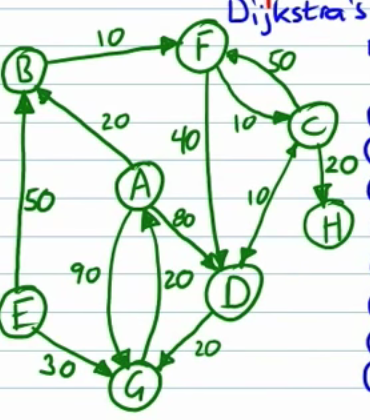
\includegraphics[scale=0.3]{dij.png}
\end{center}

4.1 (20 \%) Complete, por favor, la siguiente tabla, usando
el algoritmo de Dijkstra para encontrar el camino más corto
del punto A a todos los demás. En la tabla, la palabra ``a'' significa ``hasta''.

{\footnotesize
\begin{center}
\begin{tabular}{| c | c | c | c | c | c | c | c | c |}
\hline
Paso  & a & B & C & D & E & F & G & H \\
\hline
1 &  A  & $20$,A  & $\infty$  & $80$, A  & $\infty$   & $\infty$  & $90$, A  & $\infty$  \\
\hline
2 &  B  & $20$,A  &  $\infty$  & $80$, A  & $\infty$  & $30$,B  & $90$,A   & $\infty$  \\
\hline
3 &   &   &   &   &   &   &   &   \\
\hline
4 &   &   &   &   &   &   &   &   \\
\hline
5 &   &   &   &   &   &   &   &   \\
\hline
6 &   &   &   &   &   &   &   &   \\
\hline
7 &   &   &   &   &   &   &   &   \\ 
\hline
8 &   &   &   &   &   &   &   &   \\ 
\hline
\end{tabular}
\end{center}
}

4.2 (10 \%) ¿Cuál es el camino más corto de A a G?\\

  \_\_\_\_\_\_\_\_\_\_\_\_\_\_\_\_\_\_\_\_


\section{Búsqueda local 20\%}
El problema de las \textit{N reinas} consiste en ubicar
$N$ reinas en un tablero de ajedrez de tal forma que no
se ataque ninguna de ellas. Como un ejemplo, en el siguiente
tablero se han colocado las reinas de tal forma que no se atacan.

\begin{center}
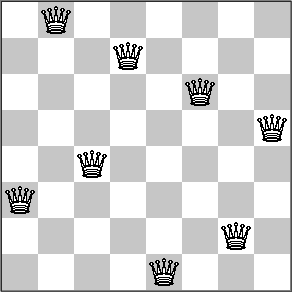
\includegraphics[scale=0.3]{8qsolved.png}
\end{center}

Una forma en que podemos describir el tablero anterior es decir que
el costo heurístico es $0$ porque hay $0$ pares de reinas que se atacan
una con la otra. Podemos generalizar esta idea para decir que el costo
heurístico de un tablero de $n$ reinas es igual al número de reinas
que atacan directa o indirectamente (o sea, como si las reinas pudieran
saltar unas a las otras) unas con otras. Considere, como un ejemplo, el
siguiente tablero del problema de las $5$ reinas. En este tablero hay $5$
pares de reinas que se atacan unas con otras y por esa razón el costo
heurístico del tablero es de $5$.

\begin{center}
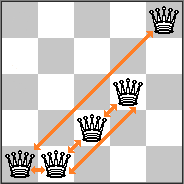
\includegraphics[scale=0.6]{5qexample.png}
\end{center}

Podemos calcular el costo heurístico facilmente si representamos un
tablero como un arreglo, donde el índice es la columna y el valor en el
arreglo es la fila. El tablero anterior sería
$[0,0,1,2,4]$. El siguiente algoritmo \textbf{calcula el costo heurístico de
un tablero de $n$ reinas}.

{\small
\begin{verbatim}
01 public static int getHcost(int[] board){
02  int h = 0;
03  for (int i = 0; i < board.length; i++){
04  // Verifica cada columna que no hemos revisado ya
05    for (int j = i+1; j < board.length; j++){ 
06    // Verifica si las reinas están en la misma fila
07    if (__________________)
08      h += 1;
09    // Obtiene la diferencia (offset) entre la columna
10    // actual  y la columna que estamos revisando 
11    int offset = j - i;
12    // Para diagonal, verifica si el valor de una columna
13    // es el mismo que el de la otra +/- el offset
14    if (board[i] == board[j] - offset 
15        || board[i] == board[j] + offset)
16      h += 1;     
17    }
18  }
19  return h;
20 }
\end{verbatim}
}

(10 \%) Complete la línea 07 del código que calcula el heurístico
para resolver las $N$ reinas con búsqueda local.\\

\_\_\_\_\_\_\_\_\_\_\_\_\_\_\_\_\_\_\_\_

%http://letstalkdata.com/2013/12/n-queens-part-1-steepest-hill-climbing/

% 01 public static int getHcost(int[] board){
% 02  int h = 0;
% 03  for (int i = 0; i < board.length; i++){
% 04  // Verifica cada columna que no hemos revisado ya
% 05    for (int j = i+1; j < board.length; j++){ 
% 06    // Verifica si las reinas están en la misma fila
% 07    if (board[i] == board[j])
% 08      h += 1;
% 09    //Obtiene la diferencia entre la columna actual (i)
% 10    //y la columna que estamos revisando (j)
% 11    int offset = j - i;
% 12    // Para diagonal, verifica si el valor de una columna es 
% 13    // el mismo que el de la otra +/- un valor de diferencia (offset)
% 14    if (board[i] == board[j] - offset 
% 15        || board[i] == board[j] + offset)
% 16      h += 1;     
% 17    }
% 18  }
% 19  return h;
% 20 }

% def get_h_cost(board):
%   h = 0
%   for i in range(len(board)):
%     #Check every column we haven't already checked
%     for j in range(i + 1,len(board)):
%       #Queens are in the same row
%       if board[i] == board[j]:
%         h += 1
%       #Get the difference between the current column
%       #and the check column
%       offset = j - i
%       #To be a diagonal, the check column value has to be 
%       #equal to the current column value +/- the offset
%       if board[i] == board[j] - offset 
%         or board[i] == board[j] + offset:
%         h += 1     
%   return h






\end{document}